% This is samplepaper.tex, a sample chapter demonstrating the
% LLNCS macro package for Springer Computer Science proceedings;
% Version 2.20 of 2017/10/04
%
\documentclass[head,11pt]{llncs}
\usepackage[utf8]{inputenc}
\usepackage[english]{babel}
\usepackage{fancyhdr}
\usepackage{hyperref}
\usepackage{lastpage}
\usepackage{graphicx}

\usepackage{hyperref}
\usepackage{caption}
\usepackage{subcaption}
 
\pagestyle{fancy}
\fancyhf{}
 
\rfoot{Page \thepage \hspace{1pt} of \pageref{LastPage}}
%
\usepackage{graphicx}
\usepackage{mathtools}
\DeclarePairedDelimiter\floor{\lfloor}{\rfloor}
\RequirePackage{algorithmic}[2009/08/24]
\RequirePackage[plain,chapter]{algorithm}
\floatplacement{algorithm}{bp}
% Used for displaying a sample figure. If possible, figure files should
% be included in EPS format.
%
% If you use the hyperref package, please uncomment the following line
% to display URLs in blue roman font according to Springer's eBook style:
% \renewcommand\UrlFont{\color{blue}\rmfamily}
\usepackage{amssymb,amsmath}
\setcounter{secnumdepth}{3}

\begin{document}

%
\title{Knowledge Graph - Entity Description Generation - UI Report}
%
%\titlerunning{Abbreviated paper title}
% If the paper title is too long for the running head, you can set
% an abbreviated paper title here
%
\author{Nabil Kazi (6850460)}
%
% First names are abbreviated in the running head.
% If there are more than two authors, 'et al.' is used.
%
\institute{University of Paderborn}
%
\maketitle              % typeset the header of the contribution
%
\section{User Interface}
\label{sec:intro}
The User interface (UI) is created using Reactjs\footnote{\url{https://reactjs.org}} along with the Axios Framework\footnote{\url{https://www.npmjs.com/package/axios}}.The UI enables the user to search for an entity and generate the description from a selected database (DBpedia/ Wikidata) respectively.Additionally allows to download the generated summary as PDF.




\subsection{Approach}
\begin{figure}
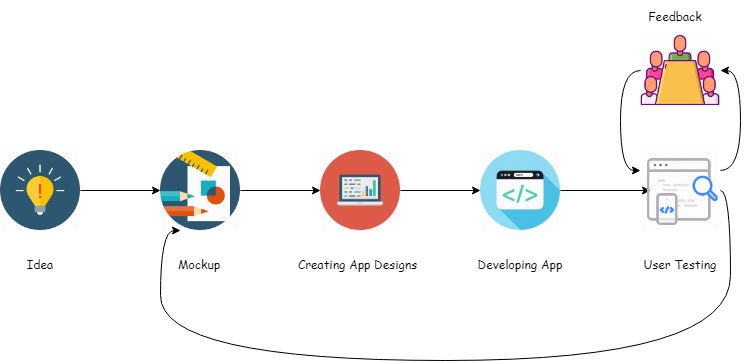
\includegraphics[width=120mm]{figures/ui process.png}
\caption{UI Waterfall Model process}
\label{ui process}
\end{figure}

UI was designed by considering the UI Waterfall model as shown in the Figure \ref{ui process}, Which roughly started with pitching in ideas and putting them together in to a presentable Mockup UI,then by designing using tools like Visual Studio Code\footnote{\url{https://code.visualstudio.com}} as the code editor and Reactjs for the front end design (Javascript, HTML, CSS).Next ,the app was developed and finally,tested after which feedback and suggestion were made and re designed accordingly.



\subsection{Prototype/Mock up Design}
This phase consisted of making a mock up version of how the UI will possibly look like initially.This was done using online tool MockFlow\footnote{\url{https://mockflow.com}} as shown in Figure \ref{ui mockup}.


\begin{figure}
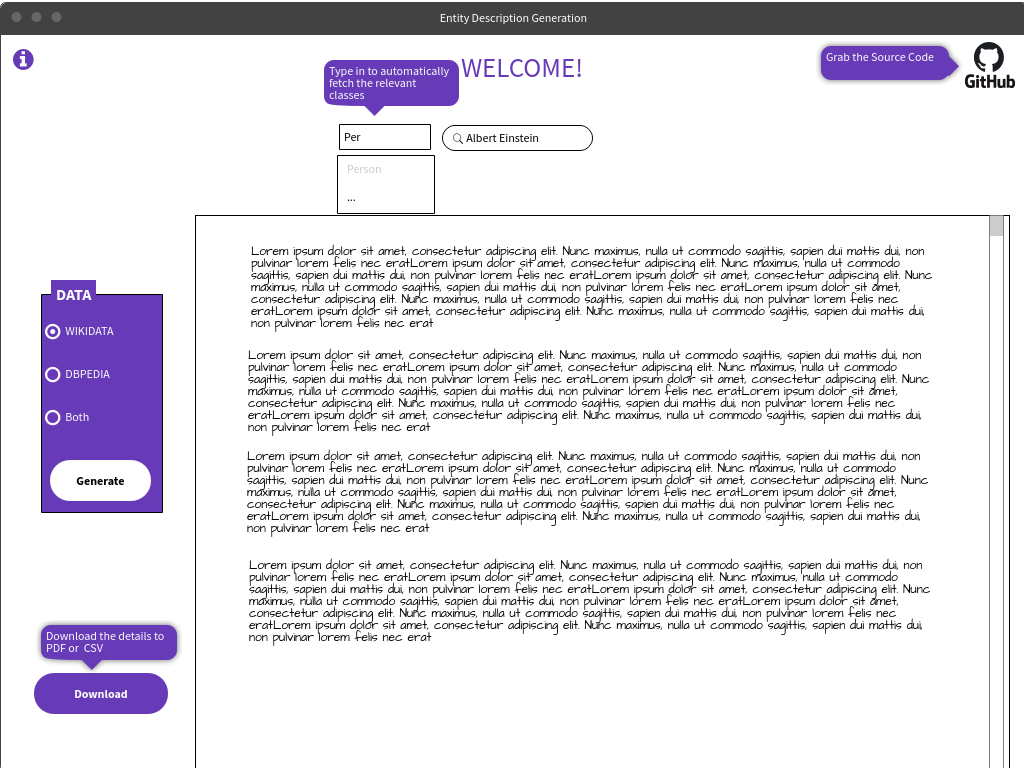
\includegraphics[width=120mm]{figures/mockup.png}
\caption{User Interface Mockup}
\label{ui mockup}
\end{figure}


\subsection{Components}
The interface is made of one main component and four sub components.
\begin{itemize}
\item Main Component: calls and displays all sub components
\item Sub Component: The components were divided in a such so that they can be edited easily independently to interact with each other and at the same time,all components are interlinked to each other.
\begin{enumerate}
\item Download Component(download.jsx).
\item Generate Component(gen.jsx).
\item Navigation Component(nav.jsx).
\item Search Component (search.jsx).
\end{enumerate}

\end{itemize}

All the sub components will be discussed below.



\subsubsection{Navigation Component}
\paragraph{}
It contains the GitHub button directing to the new and improved LD2NL Extension\footnote{\url{https://github.com/aakash2000/LD2NL_EXTENSION}} and title of the app.

\subsubsection{Search Component}
\paragraph{}
Takes an entity from the user via search bar ,while typing the user is also provided with five auto complete suggestions received by the DBpedia Lookup API\footnote{\url{https://wiki.dbpedia.org/lookup}} every time a new letter is entered as shown in Figure \ref{fig:auto}.

\begin{figure}[h!]
\centering
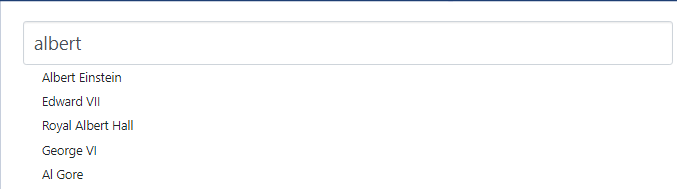
\includegraphics[width=100mm]{figures/auto.png}
\caption{Auto-Complete in progress while searching for "Albert Einstein"}
\label{fig:auto}
\end{figure}


\subsubsection{Generate Component}
\paragraph{}
The main sub component of the UI where summary is generated and displayed on UI.

\paragraph{\textbf{Entity Pronunciation play button}}
Display a play button next to search entity and pronounces if the entity is available in Knowledge Graph returned from the backend as shown in Figure \ref{fig:sound}.

\begin{figure}[h!]
\centering
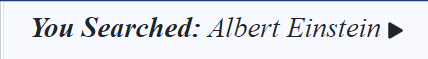
\includegraphics[width=100mm]{figures/sound.png}
\caption{Auto-Complete in progress while searching for "Albert Einstein"}
\label{fig:sound}
\end{figure}

\paragraph{\textbf{Retrieving Wikidata Entity ID:}}
 Using the Wikidata API\footnote{\url{https://www.wikidata.org/w/api.php}} which return a json format file through which I extracted some details like entity ID,label and short description. 


\paragraph{\textbf{Shortened Entity name:}}
It also handles entity name who name are shortened in either DBpedia or Wikidata due to being a long name.For example ,Sachin Dev Burman URL was shortened to \url{www.dbpedia.org/page/S._D._Burman} but our code returned URL with full name  due to which it was not able to hit an entity at the backend code, this was solved by using the redirect-checker API\footnote{\url{https://api.redirect-checker.net}}  which return the actual last redirect url for that entity.

\paragraph{\textbf{Similar Entities:}}
Additionally it provides Similar Entities when compared to original searched Entity.
The Similar Entities are displayed in a separate tab in this component and are retrieved from backend as shown and elaborated in Section 5.4 Generation of Similar Entities (Have to properly connect/ref it) 


\subsubsection{Download Component}
\paragraph{}
The component where information such as entity name, what database to get the summary and generated summary are written into the PDF file.
In the first release, a particular summary after being generated and downloaded it showed in an unformatted text file as shown in Figure \ref{fig:sub1}. A more suitable option was provided for presenting the summary in a more formatted and pleasant way as shown in Figure \ref{fig:sub2}. This was achieved by rendering the PDF on the fly ,which creates the base structure of the PDF Files as soon as the website loads and then enters other information such as which is selected DBpedia and/or Wikidata and whether the search entity has an image or not.All text with in the PDF is also selectable.Figure \ref{fig:file} shows the major difference as to what was achieved in the final release. 
\begin{figure}[h!]
	\centering
	\begin{subfigure}{.6\textwidth}
		\centering
		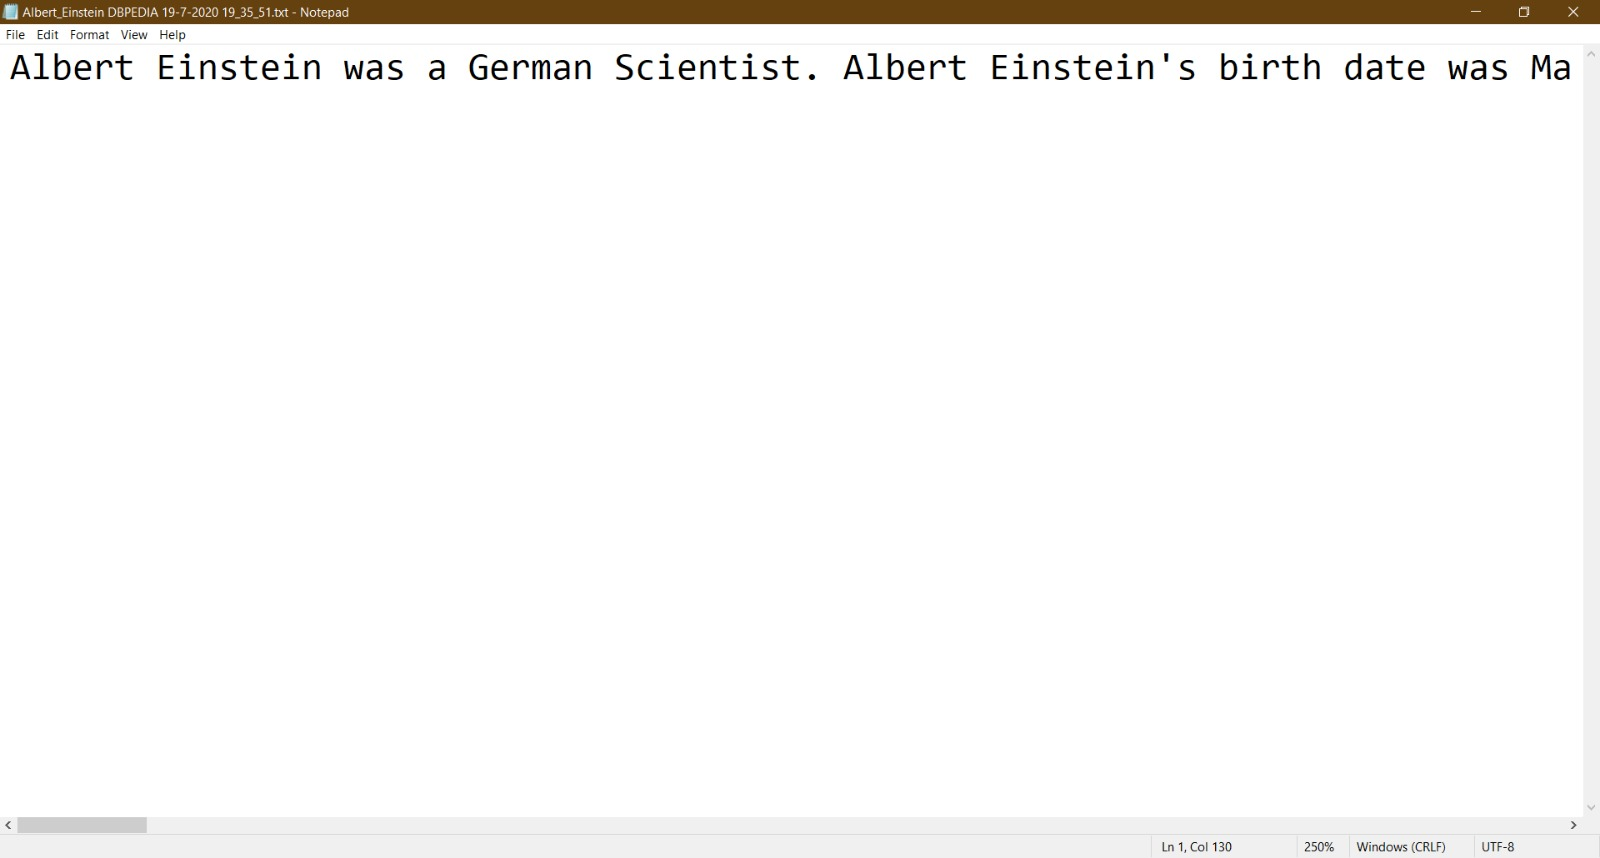
\includegraphics[width=.8\linewidth]{figures/old text.jpeg}
		\caption{Text File Format(First Release)}
		\label{fig:sub1}
	\end{subfigure}%
	\begin{subfigure}{.4\textwidth}
		\centering
		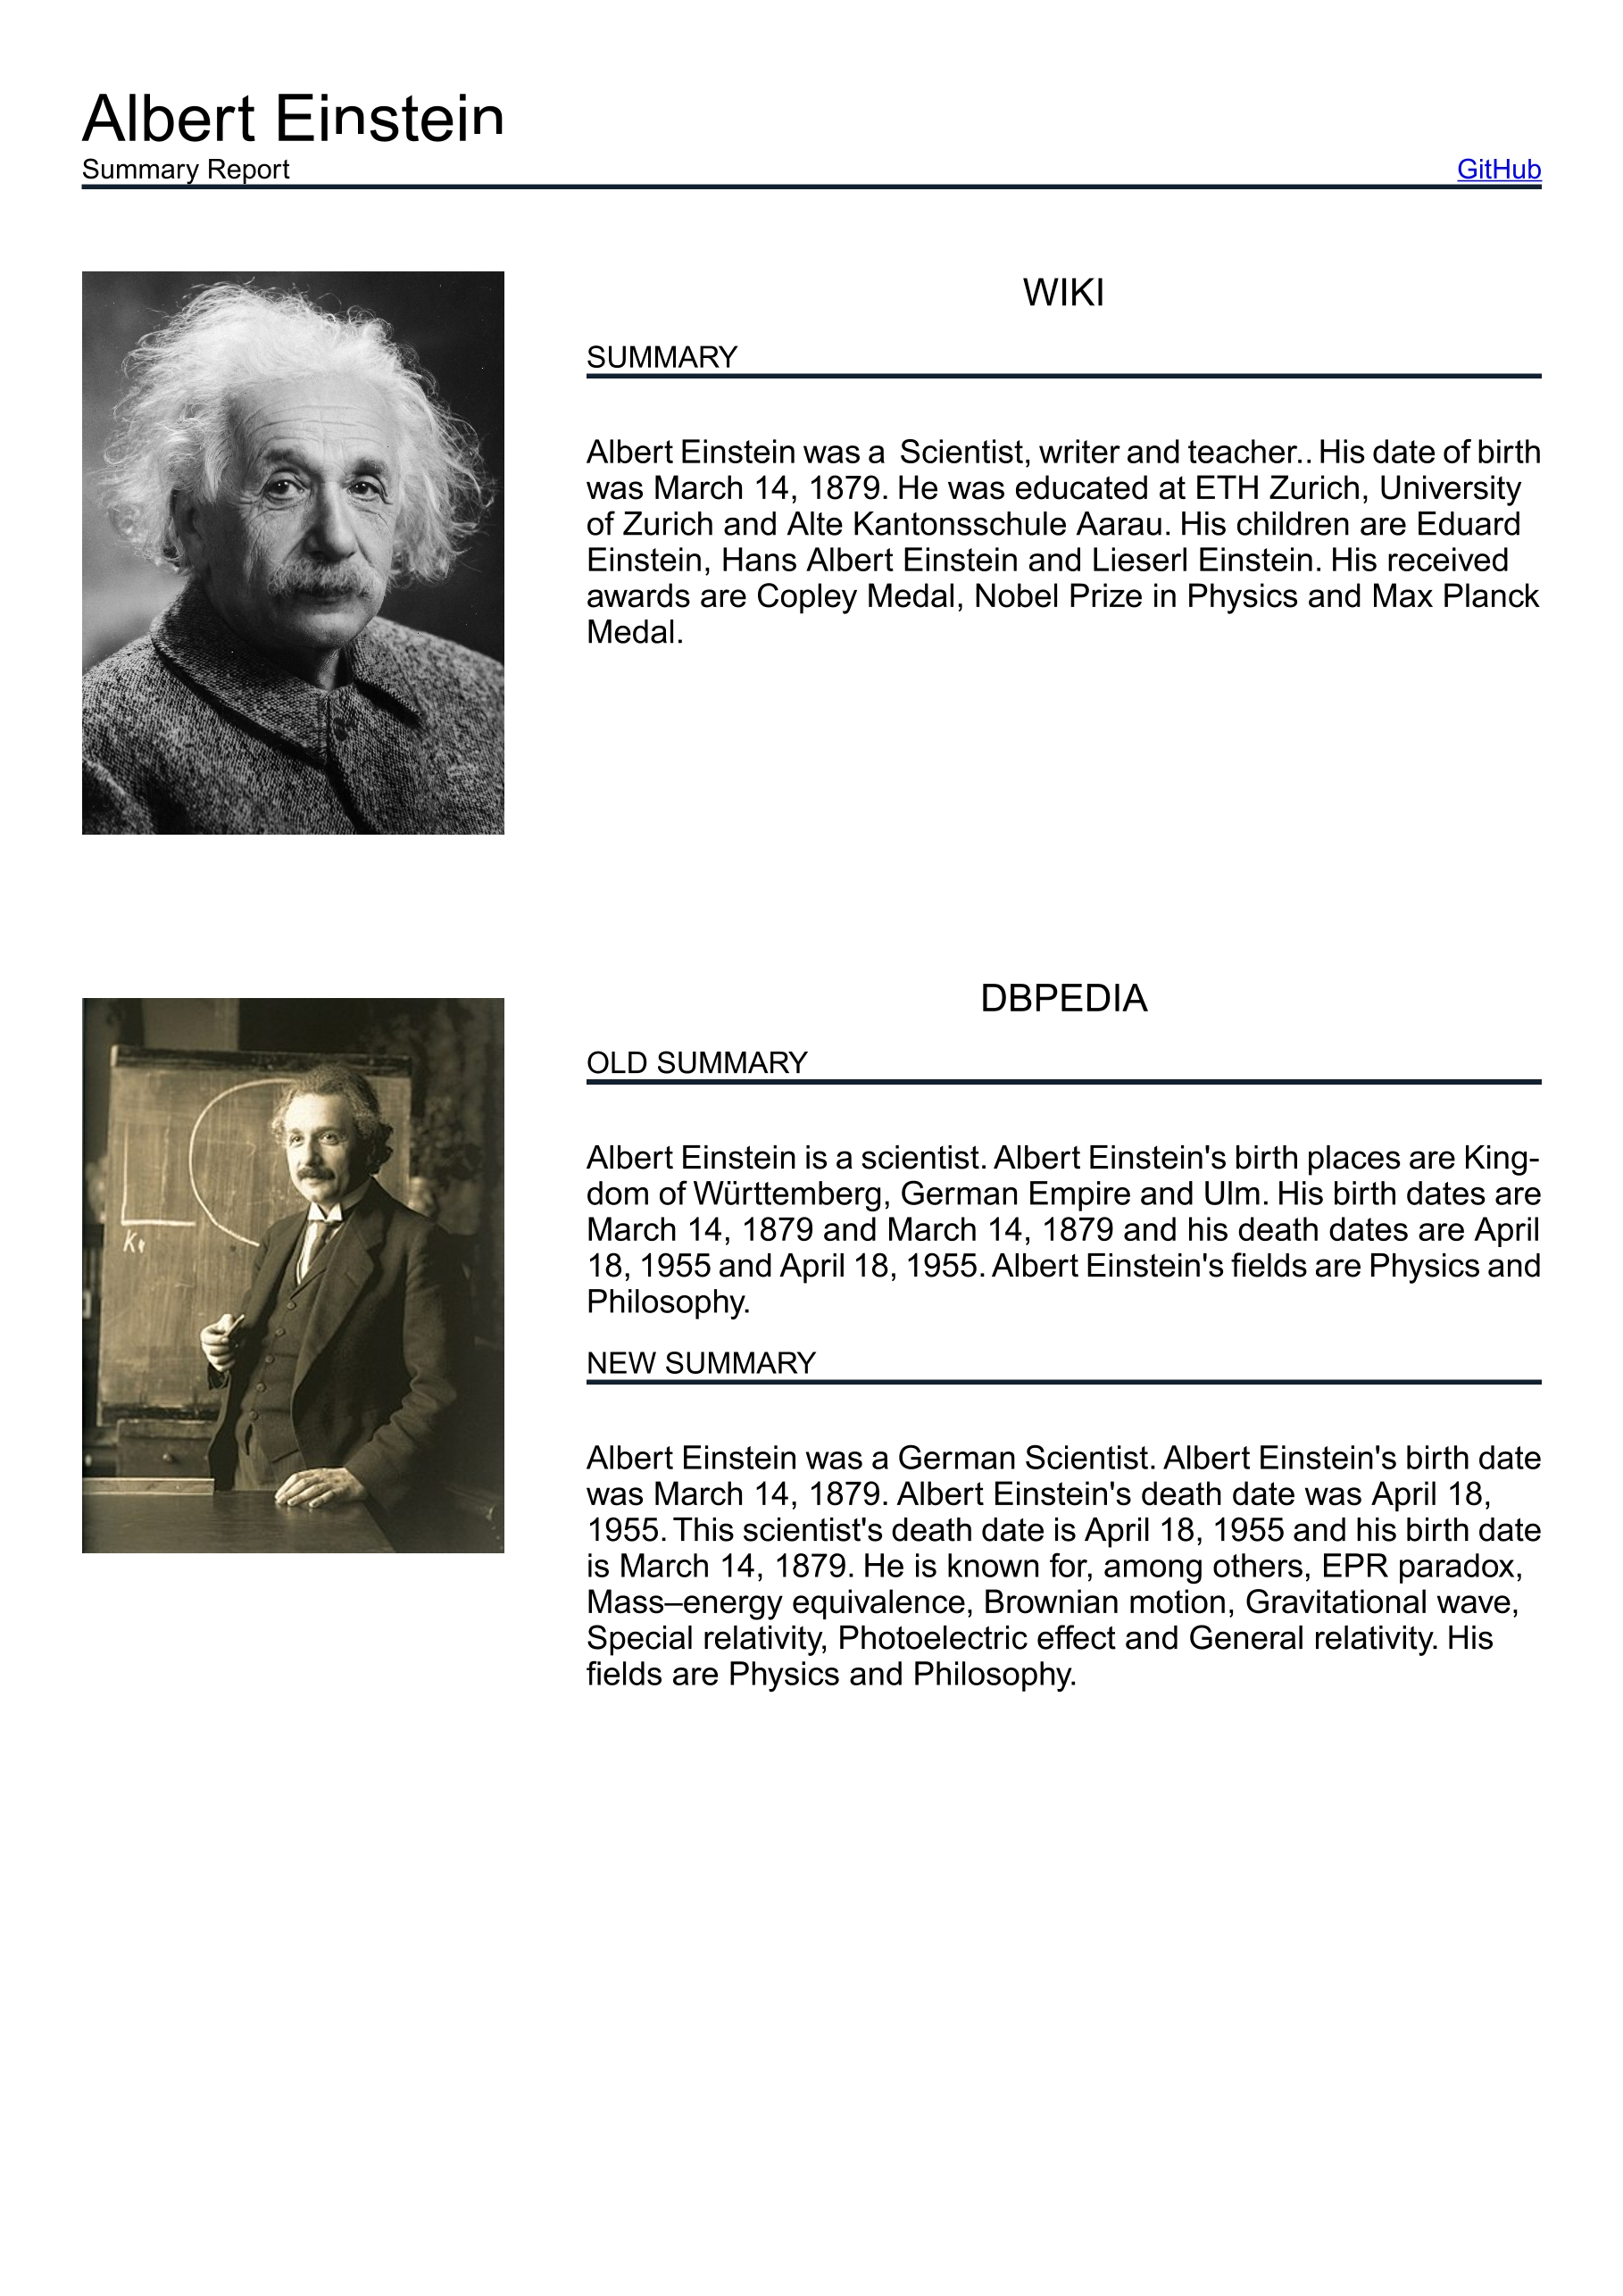
\includegraphics[width=.8\linewidth]{figures/albert.jpg}
		\caption{PDF Format(Final Release)}
		\label{fig:sub2}
	\end{subfigure}
	\caption{Generated Summary available as download}
	\label{fig:file}
\end{figure}


\section{Connection between Frontend and Backend}
Finally,the UI is connected at two different places at the backend which is Old/Original LD2NL program\footnote{\url{https://github.com/akshay05091992/Old_Version}} and New LD2NL along with Wikidata program\footnote{\url{https://github.com/aakash2000/LD2NL_EXTENSION}}.Figure \ref{fig:pgov} illustrates the Overview of the Project Architecture.

\begin{figure}
\centering
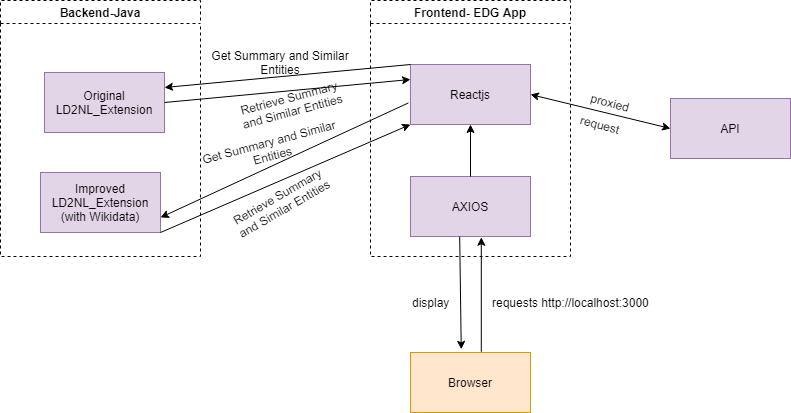
\includegraphics[width=100mm]{figures/pg overview.png}
\caption{Project Overview Architecture}
\label{fig:pgov}
\end{figure}

\newpage
\section{Locally Setup Project}
The project can be locally setup by following the below steps:
\begin{enumerate}
\item git clone \url{https://github.com/akshay05091992/Old_Version.git}
\item Run Old Version in the preferred software either IntelliJ IDEA\footnote{\url{https://www.jetbrains.com/idea}} or Eclipse IDE\footnote{\url{https://www.eclipse.org/ide}} and start the tomcat server\footnote{\url{https://tomcat.apache.org}}.
\item git clone \url{https://github.com/aakash2000/LD2NL_EXTENSION.git}
\item  Run LD2NL EXTENSION in the preferred software either IntelliJ IDEA or Eclipse IDE and start the tomcat server.
\item git clone \url{https://github.com/akshay05091992/Entity-Description-Generation-UI.git}.
\item cd Entity-Description-Generation-UI
\item npm clean-install
\item npm start
\item wait for npm\footnote{\url{https://www.npmjs.com}} to compile and deploy on localhost.
\item Once compiled, the project is available and the UI can be reached by hitting the URL \url{http://localhost:3000} on the preferred browser.


\end{enumerate}









\end{document}